\chapter{Conception et réalisation de l'application Health+}

Ce chapitre est réservé à l'application e-santé mobile réalisée dans le cadre de ce projet. Il est organisé en quatre parties. La première partie présente en détails l'approche PPAMH. La deuxième montre les résultats d'analyse et de conception avant de présenter l'étude technique dans la troisième partie. Enfin l'application Health+ est présentée dans la dernière partie.

\section{Approche PPAMH}

PPAMH est une approche qui consiste à préserver la vie privée dans les applications e-santé mobiles. Cette solution vise à aider les patients à exprimer leurs préférences en ce qui concerne la divulgation de leurs données sensibles. Ces préférences seront transformées par la suite en politiques de privacy qui doivent être respectées par les tiers à l'aide d'un contrat $[8]$.

\subsection{Architecture de PPAMH}

Cette section décrit l'architecture générale de la solution PPAMH. Elle est constituée de composants suivants $[8]$:

\vspace{6pt}
\paragraphmark

\textbf{PPIAMH}: \footnote{Privacy-Preserving Intelligent Application for Mobile Healthcare} est une application mobile intelligente dont les objectifs sont:

\vspace{6pt}
\paragraphmark

\begin{itemize}
	\item Déterminer le type de groupe: le groupe est désigné par un questionnaire simple que le patient/professionnel de la santé doit remplir.
	\item Prévoir les préférences de confidentialité du patient/professionnel de santé concernant les informations sensibles qu'il veut dévoiler et à qui ces informations sont divulguées.
	\item la compréhension de politiques de confidentialité par le patient est la première étape vers un niveau plus élevé de protection de la vie privée. Ainsi, la solution a pour objectif de présenter et de faciliter la compréhension des politiques de confidentialité en utilisant des schémas par exemple, car les utilisateurs en particulier les patients ne sont pas souvent disposés à lire des politiques de confidentialité qui sont complexes et longues.
\end{itemize}

\vspace{8pt}
\paragraphmark

\textbf{Une partie de confiance}: une autorité de confiance dont les principaux objectifs sont:

\vspace{6pt}
\paragraphmark

\begin{itemize}
	\item Transformer les préférences des patients en politiques de privacy.
	\item Fournir un contrat qui doit approuvé par les systèmes e-santé et les fournisseurs de Cloud.
\end{itemize}

\vspace{8pt}
\paragraphmark

\textbf{Un accord}: établi entre l'autorité de confiance et les systèmes e-santé (ou les fournisseurs de Cloud). Il les oblige à respecter les préférences des patients et d'autres parties des politiques de privacy afin d'éviter tout conflit.

\subsection{Processus d'affectation des politiques de privacy}

Pour affecter des politiques de confidentialité adéquates au bon patient, quatre principales étapes sont effectuées. Ces étapes sont décrites dans la figure \ref{ppamh}:

\vspace{8pt}
\paragraphmark

\begin{figure}[!ht]
\begin{center}
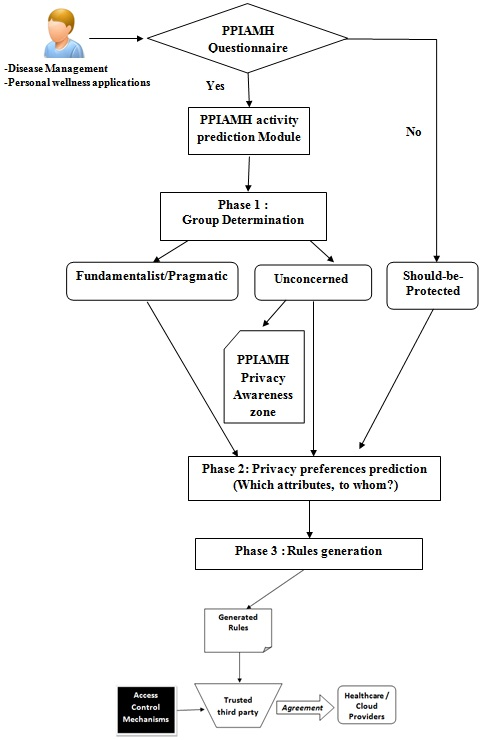
\includegraphics[scale=0.72]{ppamh.jpg}
\caption{Schéma de PPAMH $[8]$}
\label{ppamh}
\end{center}
\end{figure}

Comme le montre la figure \ref{ppamh}, le groupe auquel appartient le patient est défini dans la Phase 1. Ensuite, dans la phase 2, le système prédit son comportement et lui permet de faire ses préférences d'une manière simple. Ensuite, un ensemble de règle sont générés dans la phase 3. Ces règles sont utilisées conjointement avec le type de groupe pour générer des politiques de confidentialité adéquates $[8]$.

\subsubsection{Phase 1 - Détermination du groupe}

L'application intelligente PPIAMH propose aux patients (dans un bon état) un questionnaire simple. Les patients sont invités à répondre à des questions ordinaires en prenant en considération que les niveaux d'éducation, l'âge et l'état des patients sont différents. À partir des réponses d'un patient, on déduit son groupe $[8]$.

\vspace{6pt}
\paragraphmark

On distingue quatre types de groupes $[8]$:

\vspace{6pt}
\paragraphmark

\begin{itemize}
	\item Le groupe fondamentaliste (The Fundamentalist group): Des patients (utilisateurs des applications mobiles ou des patients à l'hôpital) qui se méfient des institutions de santé, des fournisseurs de Cloud et ils préfèrent contrôler l'accès à leurs renseignements personnels.
	\item Le groupe pragmatique (The Pragmatic group): Des patients (utilisateurs des applications mobiles ou des patients à l'hôpital) qui considèrent que la confiance aux tiers (institutions et fournisseurs de Cloud) ne devrait pas être donnée librement.
	\item Le groupe des indifférents (The Unconcerned group): Des patients (utilisateurs des applications mobiles ou des patients à l'hôpital) qui font confiance aux organisations qui recueillent leurs renseignements personnels. Ils sont à l'aise avec les procédures organisationnelles existantes.
	\item Le groupe Devrait-être-protégé (The Should-Be-Protected group): Dans ce groupe, le patient n' est pas indifférent et en même temps, il ne peut pas prendre des décisions pour contrôler la divulgation de ses données. Par conséquent, il est automatiquement classé comme "Devrait-être-protégé". Ce groupe comprend les enfants et les patients gravement blessé (patients à l'hôpital) ou les patients atteints d'une maladie mentale critique.
\end{itemize}

\subsubsection{Phase 2 - Prédiction des préférences de confidentialité}

Après avoir déterminé le groupe auquel le patient appartient, les prochaines étapes visent à anticiper ses préférences concernant ses informations sensibles (quelle donnée à divulguer et à qui) $[8]$.

\subsubsection{Phase 3 - Génération des règles}

Les préférences de confidentialité sont exprimées dans des politiques normalisées et présentées de manière simple pour être comprises par les tiers $[8]$.

\subsubsection{Phase 4 - Mise de l'accord de confidentialité}

Un accord adressé à des tiers, y compris les fournisseurs de Cloud et les institutions de santé. L'objectif de cet accord est de les obliger à respecter les préférences du patient $[8]$.

\section{Analyse et conception}

Dans le but de concevoir un système extensible, évolutif, modulaire et orienté objet, le formalisme UML \footnote{Unified Modeling Language} est imposé comme l’outil le plus approprié pour ce projet. En effet, le langage de modélisation UML permet de mener la phase de conception tout en bénéficiant de la puissance et de la simplicité de ses diagrammes.

\subsection{Diagrammes de cas d’utilisation du système}

Un cas d’utilisation est une collection de scénarii qui décrit la façon dont un ou plusieurs acteurs interagissent avec un système pour atteindre un but. Les scénarios prennent la forme d’une description textuelle d’actions ou d’interactions entre un ou des acteurs et le système modélisé (Use Case).

\subsubsection{Pour un patient}

Pour bénéficier des fonctionnalités de l’application le patient doit premièrement s’authentifier. Cette authentification peut se faire selon deux manières différentes: soit à l’aide d’un login et un mot de passe ou via une connexion à travers un réseau social dont le patient est déjà inscrit (figure \ref{patient}).

\begin{figure}[!ht]
\begin{center}
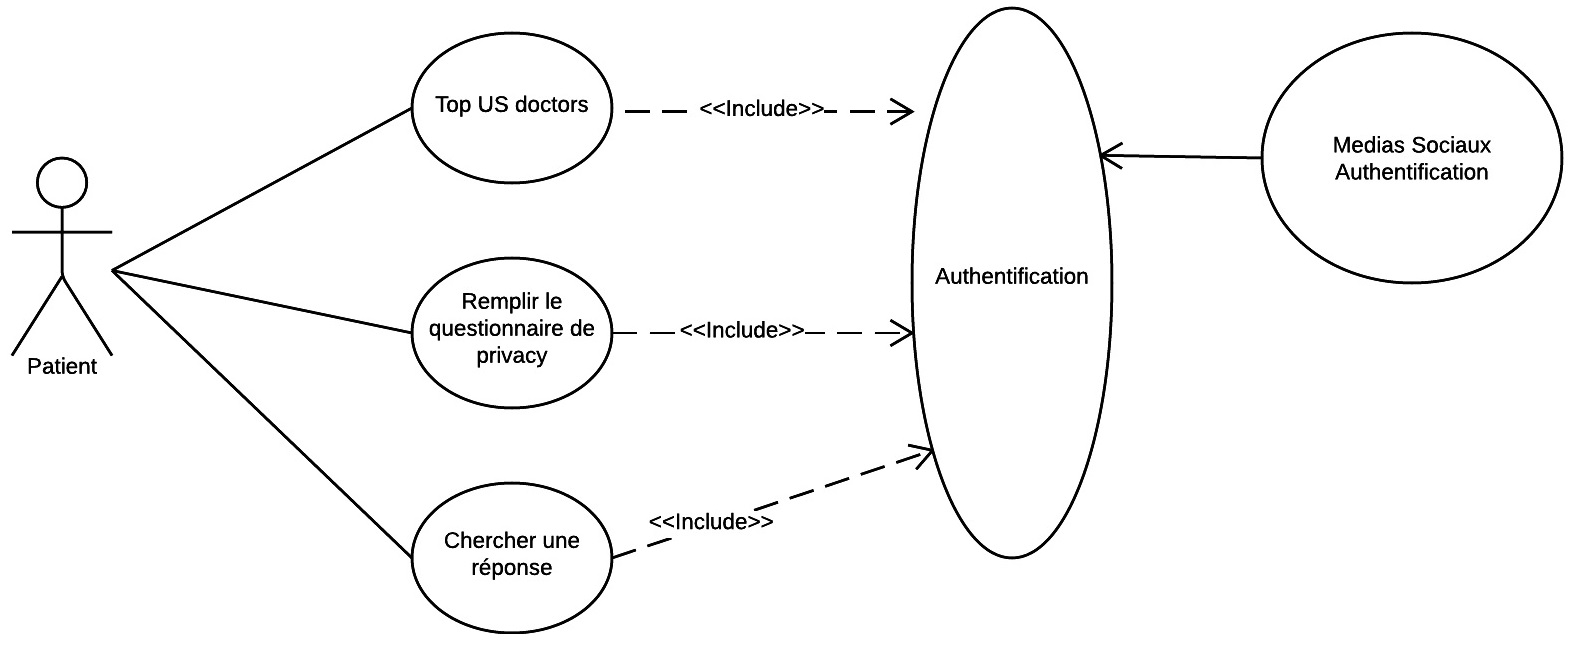
\includegraphics[scale=0.4]{patient.jpg}
\caption{Diagramme de cas d'utilisation d'un patient}
\label{patient}
\end{center}
\end{figure}

Après la première authentification réussie, le patient doit répondre au questionnaire pour déterminer le niveau de privacy à mettre en place. Ensuite il peut consulter les questions et les réponses ou bien voir un médecin dans notre liste de top US docteurs comme indiqué par la figure \ref{patient}.

\subsubsection{Pour l'administrateur}

\begin{figure}[!ht]
\begin{center}
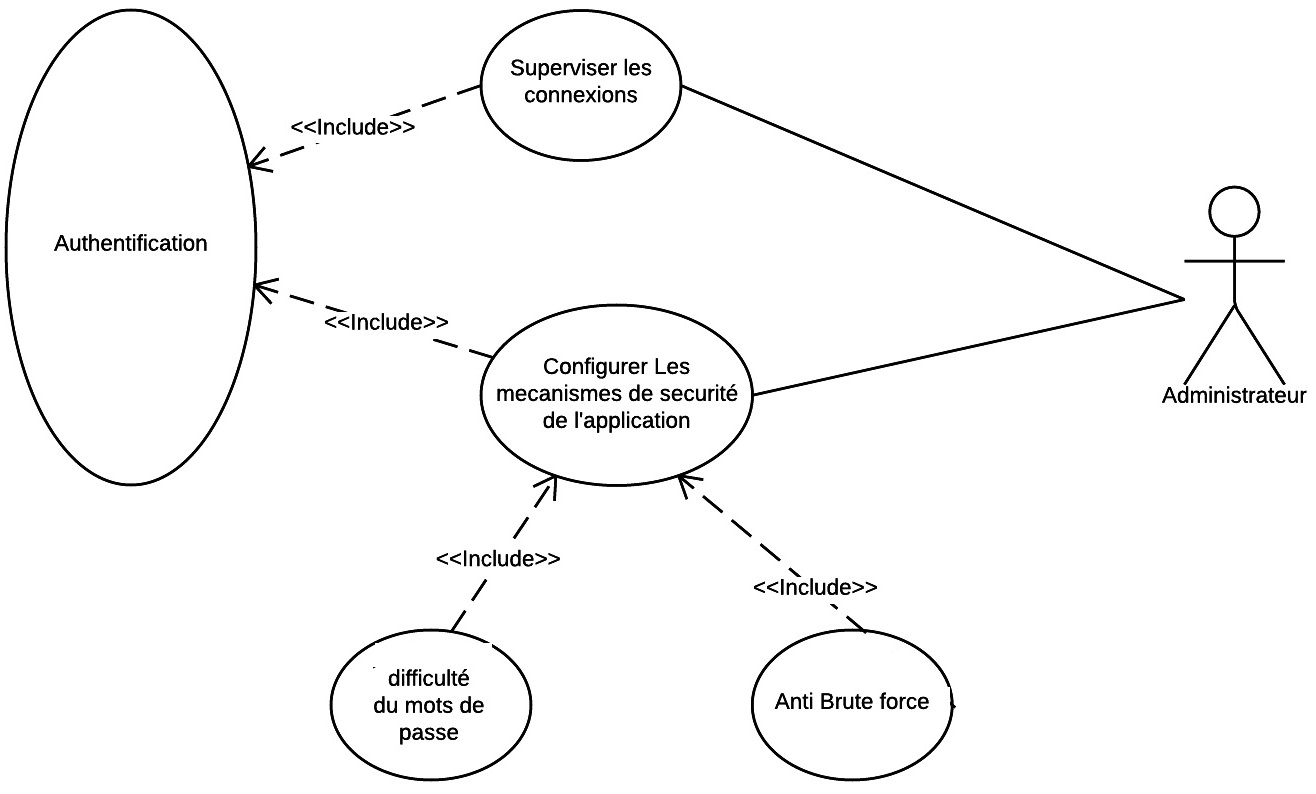
\includegraphics[scale=0.42]{admin.jpg}
\caption{Diagramme de cas d'utilisation de l'administrateur}
\label{admin}
\end{center}
\end{figure}

Un administrateur supervise les actions d’authentification des patients depuis une interface d’administration, il peut aussi configurer les paramètres de sécurité de l’application comme cela est indiqué dans la figure \ref{admin}.

\subsection{Diagramme de séquences}

Les diagrammes de séquences sont la représentation graphique des interactions entre les acteurs et le système selon un ordre chronologique dans le langage UML.

\subsubsection{Pour le mécanisme d'authentification}

La figure \ref{seq} présente le diagramme de séquences pour le mécamisme d'authentification composé de cinq étapes suivants:

\vspace{6pt}
\paragraphmark

\begin{figure}[!ht]
\begin{center}
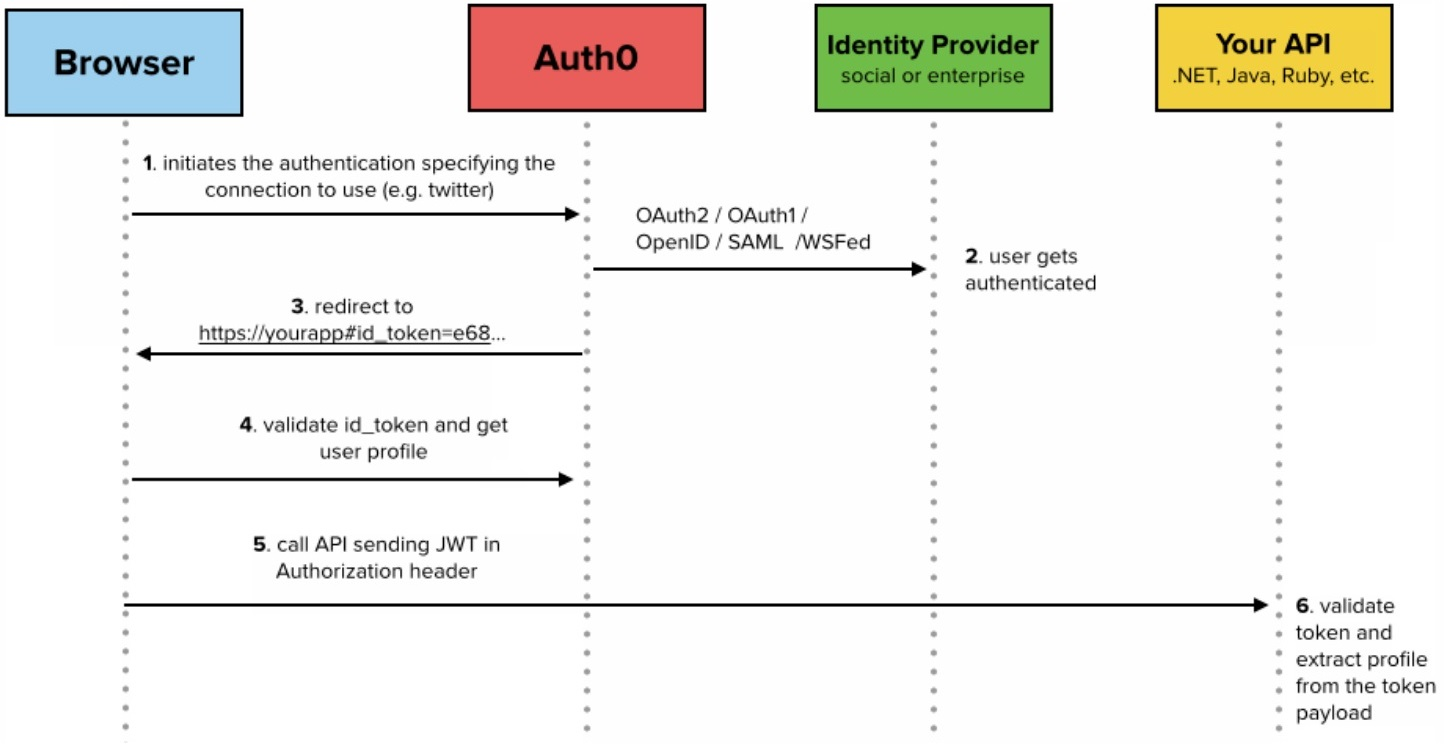
\includegraphics[scale=0.42]{seq.jpg}
\caption{Diagramme de séquences d'authentification $[W10]$}
\label{seq}
\end{center}
\end{figure}

\begin{itemize}
	\item Etape 1: L'interface d'autentificatiosn spécifie la connexion à utiliser (par exemple twitter);
	\item Etape 2: Auth0 va demander au Provider le token avec des droits d’accès précis à travers les protocoles OAuth;
	\item Etape 3: Le Provider donnera l’autorisation sous forme de token d'accès;
	\item Etape 4: la redirection va être faite pour valider le token et avoir les informations concernant le profil du patient;
	\item Etape 5: l’utilisateur est authentifié et les informations relatives au token en question seront extraites pour une utilisation ultérieure.
\end{itemize}

\section{\'Etude technique}

L'étude technique est une étape nécessaire pour une réalisation rigoureuse d’une application conforme aux résultats d'analyse et de conception. Dans cette partie, les outils adéquats aux besoins sont déterminés afin d'aboutir à une application moderne avec un design intuitif, innovant et accessible pour rendre l'expérience des utilisateurs plus agréable.

\subsection{Choix de la technologie mobile}

Le développement des applications mobiles peut être effectué selon plusieurs démarches comme indiqué ci-dessus:

\vspace{6pt}
\paragraphmark

\begin{itemize}
	\item Développement Native en utilisant un SDK du système d’exploitation mobile exemple Android SDK, IOS SDK à l’aide du langage Objective-C ou dernièrement le langage Swift;
	\item Site web mobile: Un site web responsive adapté aux navigateurs mobiles;
	\item Une application web: Une esthétique qui ressemble à une application mobile native comme Facebook , Linkedin et Twitter;
	\newpage
	\item Applications Hybrides: Ces applications sont basées sur un ensemble de langages communs entre toutes les plateformes. Dans ce cas, les plus souvent utilisés sont les langages issus du Web : HTML, CSS, JavaScript. Une application hybride, qu’elle soit destinée à Android ou un iPhone, sera donc construite sur ces technologies standards, connues et exécutées par tous les smartphones du marché. La dépendance à une plateforme spécifique est perdue mais cela induit une réduction du temps (et donc des coûts) liée au développement ainsi qu’une facilité de maintenance. Il est également à noter que certaines portions sont réalisées en code natif pour accéder aux fonctions avancées du téléphone (notifications Push par exemple), rendues accessibles par des « ponts » entre la partie native et la partie hybride. Le développement hybride tire donc partie du meilleur des deux mondes.
\end{itemize}

\subsubsection{\'Etude comparative}

Le tableau ci-dessous présente une étude comparative des différentes démarches possibles pour le développement mobile:

\begin{figure}[!ht]
\begin{center}
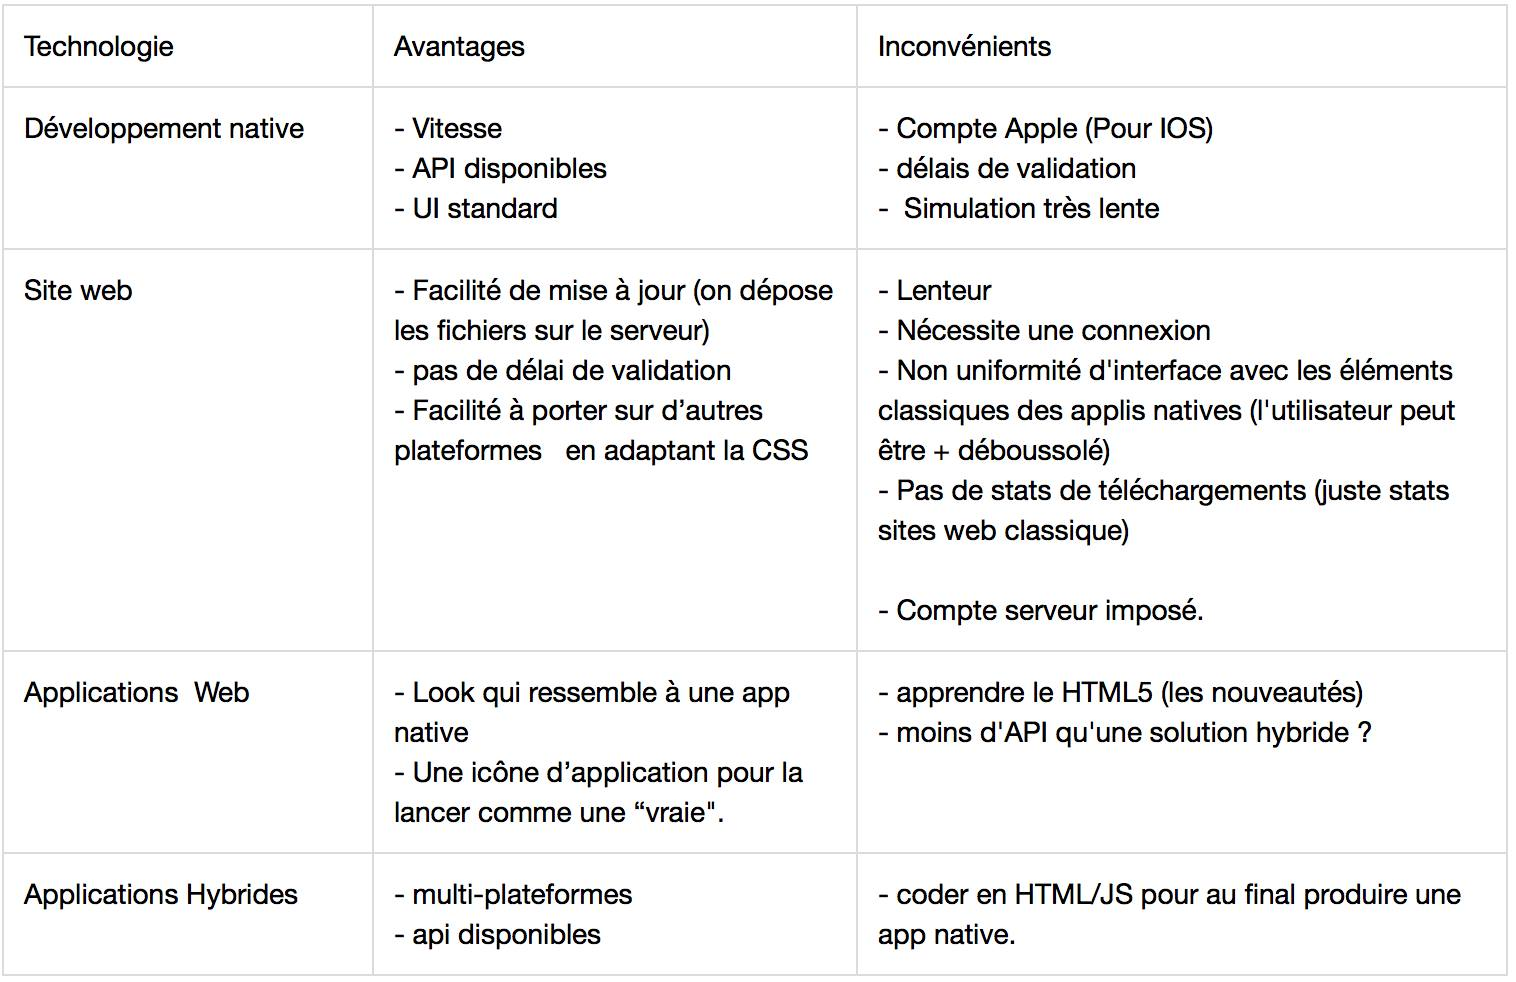
\includegraphics[scale=0.32]{etude.jpg}
\end{center}
\end{figure}

D’après cette étude (tableau ci-dessus), le développement hybride est le choix le plus adapté pour réaliser une application e-santé mobile conforme aux besoins décrits dans les étapes d'analyse et de conception.

\newpage

\subsubsection{Choix du framework}

\textbf{PhoneGap}: est un framework libre basé principalement sur HTML5, CSS3 et JavaScript qui permet le
développement multiplateforme mobile. En effet, ce framework peut être déployé sur sept plateformes différentes et il permet aussi un accès aux fonctions de bas niveau. En effet son fonctionnement basé sur des outils de développement web, permet au programmeur d’accéder à des fonctions natives des appareils mobiles telles que la caméra, la géolocalisation, les contacts etc.

\begin{figure}[!ht]
\begin{center}
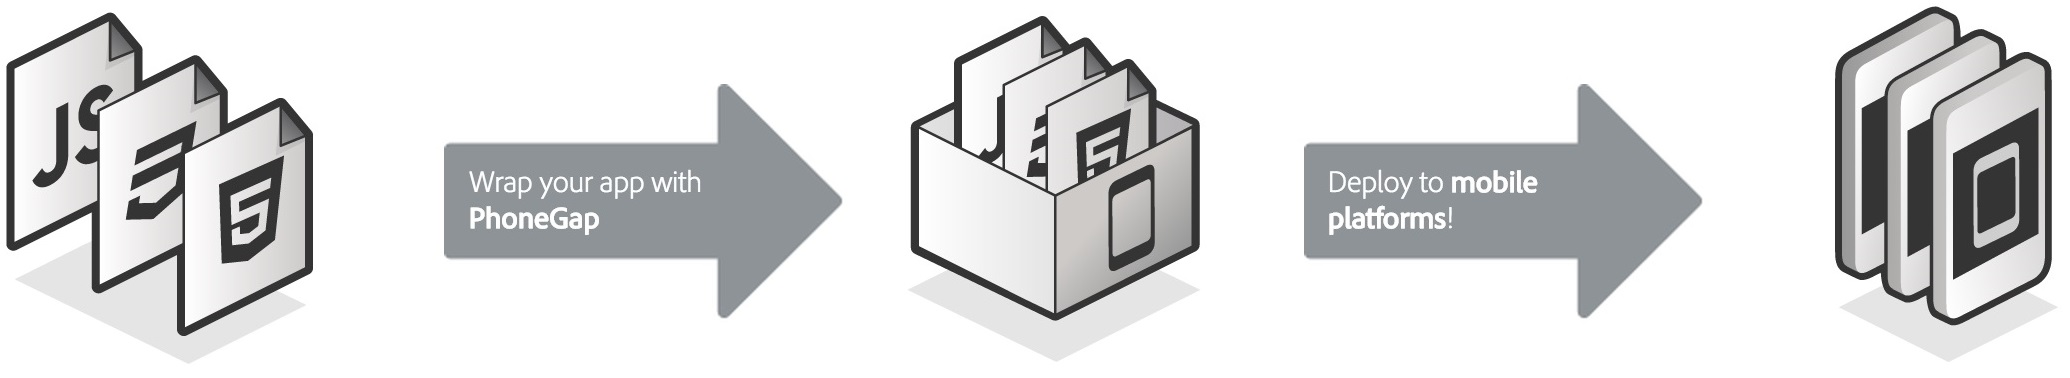
\includegraphics[scale=0.3]{p1.jpg}
\caption{Fonctionnement du framework PhoneGap $[W11]$}
\label{p1}
\end{center}
\end{figure}

Comme indiqué dans la figure \ref{p1} $[W11]$, le framework PhoneGap enveloppe des fichiers sources HTML5, CSS3 et JavaScript et permet par la suite de développer une application peut être déployée sur plusieurs plateformes.

\subsubsection{Les fonctionnalités natives supportées par PhoneGap}

PhoneGap ne peut pas accéder à toutes les fonctionnalités natives des smartphones comme nous l’avons évoqué précedemment. Le tableau ci-dessous (figure \ref{p2}) montre les fonctionnalités accessibles et celles qui ne le sont pas pour ce framework:

\begin{figure}[!ht]
\begin{center}
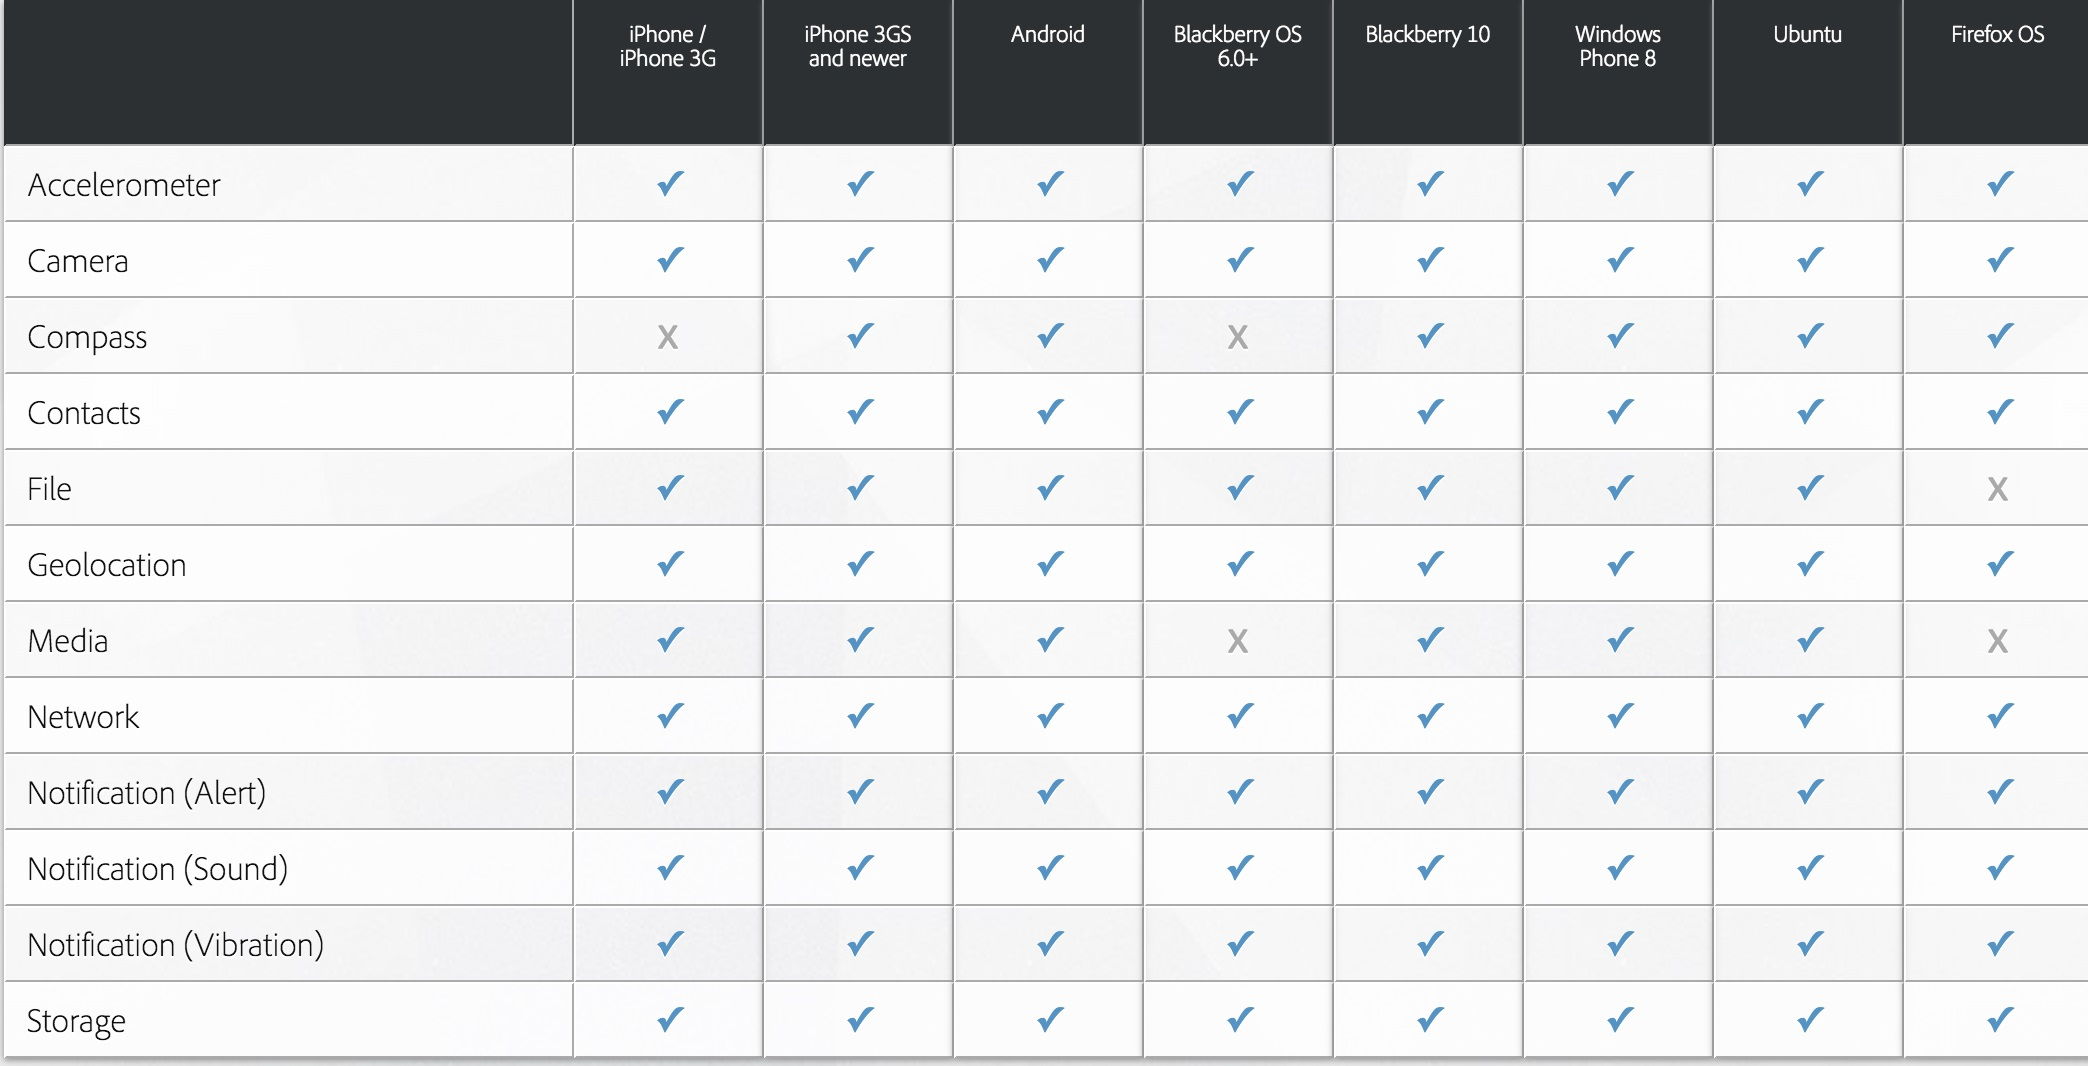
\includegraphics[scale=0.3]{p2.jpg}
\caption{Fonctionnalités supportées par le framework PhoneGap $[W12]$}
\label{p2}
\end{center}
\end{figure}

\vspace{6pt}
\paragraphmark

Dans l’ensemble, nous constatons que même si PhoneGap ne couvre pas toutes les fonctionnalités natives pour certains systèmes d’exploitation, il couvre l’intégralité de celles d’Android et d’IOS qui dominent le marché.

\vspace{6pt}
\paragraphmark

Puisque notre framework utilise le javascript comme langage de programmation, et vu qu’il n’est pas aisé de réaliser de grandes applications qui répondent à des besoins bien détaillés avec Javascript cela nécessitera l’ajout d’une couche d’abstraction MVC à l’aide d’un framework comme AngularJS.

\subsection{Framework AngularJS}

AngularJS est un framework Javascript qui permet de créer des applications web dynamiques. Ce type d'applications (souvent appelées SPA pour Single Page Application) sont de plus en plus présentes avec des périphériques connectés de plus en plus variés. Malheureusement, créer une application tenant sur une seule page n'est pas chose simple. En effet, cela requiert l’utilisation de beaucoup de Javascript et il est très difficile de bien s’organiser et d'obtenir une application maintenable et modulable ainsi. C’est ici qu’AngularJS intervient $[W13]$.

\vspace{6pt}
\paragraphmark

La figure \ref{a1} ci-dessous présente une étude comparative des frameworks javascript basée sur le nombre de lignes de code:

\begin{figure}[!ht]
\begin{center}
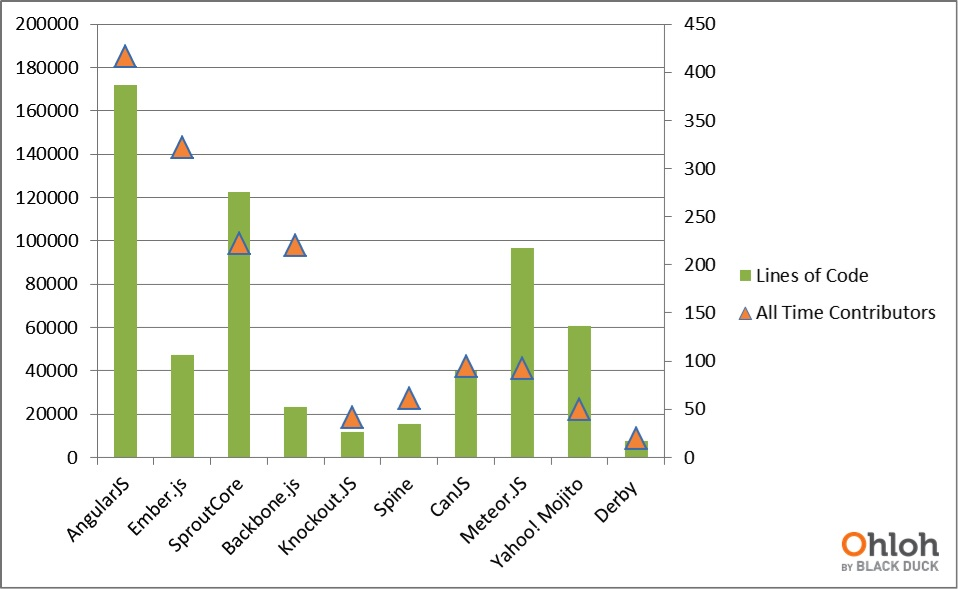
\includegraphics[scale=0.6]{a1.jpg}
\caption{\'Etude comparative des frameworks javascript basée sur le nombre de lignes de code $[W13]$}
\label{a1}
\end{center}
\end{figure}

D'après cette étude (figure \ref{a1}), le framework AngularJS est le plus prometteur coté nombre de ligne de code par contributeur.

\subsection{IONIC Framework}

IONIC est un projet open source front-end SDK pour le développement des applications mobiles hybride en utilisant seulement du HTML5. Ce framework offre une API pour le développement mobile qui optimise du HTML5, du CSS3 et des composantes Javascript afin d’obtenir des gestures et des outils pour construire des applications hybride interactive de haute qualité. Ainsi, l'un de ses avantages majeures est l'optimisation d’AngularJS ce qui prouve son utilisation dans ce projet.

\subsection{Auth0}
\label{auth0}

Auth0 est une plateforme offrant des fonctionnalités avancées permettant d'éviter les difficultés rencontrées lors de la mise en place d'un système d'authentification rigoureux. Il possède plusieurs avantages, à savoir:

\vspace{6pt}
\paragraphmark

\begin{itemize}
	\item Extensibilité : Auth0 est facilement adaptable à de nouvelles politiques d'authentification ou à de nouvelles infrastructures logicielles;
	\item Une API simple : à la fois simple et sécurisée à travers HTTPS, l'API de Auth0 permet une intégration fluide avec les autres outils utilisés au sein du projet. Elle permet d'authentifier et d'autoriser des applications et des API à travers n'importe quel fournisseur d'identité tournant sur n'importe quelle structure logicielle;
	\item Des protocoles standards : Auth0 supporte les standards de l'industrie tels que SAML, OpenID Connect, JSON Web Token, OAuth 2.0, OAuth 1.0 WS-Federation et OpenID;
	\item Scalable : la disponibilité est un point clé pour Auth0, si un utilisateur n'arrive pas à se connecter, il ne peut rien faire. C'est pour cela qu'Auth0 offre une SLA garantie quelque soit le nombre d'utilisateurs de l'application.
\end{itemize}

\vspace{6pt}
\paragraphmark

Elle offre des mécanismes de sécurité suivants $[W14]$:

\vspace{6pt}
\paragraphmark

\begin{itemize}
	\item Haute sécurité par défaut : Toutes les bonnes pratiques de la gestion des certificats et de l'authentification ont été mises en place par défaut dans Auth0 : les mots de passes ne sont jamais enregistrés en texte brut, ils sont hashés en utilisant Bcrypt. Des Web tokens JSON signés digitalement sont utilisés. Toutes les informations de configurations sensibles sont cryptées;
	\item  Un trafic crypté : toutes les intéractions en réseau entre Auth0 et ses utilisateurs ou les appareils des clients finals passent à travers SSL avec un cryptage AES à 128 bits. la connexion utilise TLS 1.2 et elle est cryptée et authentifiée en utilisant AES\_128\_GCM et emploie ECDHE\_RSA comme mécanisme d'échange de clés;
	\item Auth0 est certifié SOC 2 : Le code d'Auth0 est régulièrement audité par un organisme tiers comme liftsecurity.io et sakurity.com pour vérifier que toutes les pratiques de sécurité sont respectées et qu'aucune vulnérabilité n'est introduite.
\end{itemize}

\vspace{6pt}
\paragraphmark

Toute information enregistrée sur un compte Auth0 est privée et ne peut être accessible que par les tokens appropriés: ceux de l'utilisateur et ceux des co-admins. Aucun mécanisme de partage de configuration ou d’aucune autre information entre les comptes n’est présent $[W14]$.

\section{Réalisation}

Cette partie est consacrée à la mise en oeuvre de l'application Health+ en utilisant les outils cités dans l'étude technique.

\vspace{6pt}
\paragraphmark

Notre but est de réaliser une application mobile tout en respectant les contraintes suivantes:

\vspace{6pt}
\paragraphmark

\begin{itemize}
	\item Sécurité;
	\item Préservation de la vie privé (Privacy);
	\item Ergonomie;
	\item Multitude: Application multi-plateformes.
\end{itemize}

\subsection{Mécanisme d’authentification}

Comme indiqué à la section \ref{auth0}, nous avons intégré le système d’authentification de chez Auth0. Nous allons maintenant faire le tour de ses différentes fonctionnalités. La figure \ref{e1} montre le panneau de supervision des authentifications liées à l’application.

\vspace{6pt}
\paragraphmark

\begin{figure}[!ht]
\begin{center}
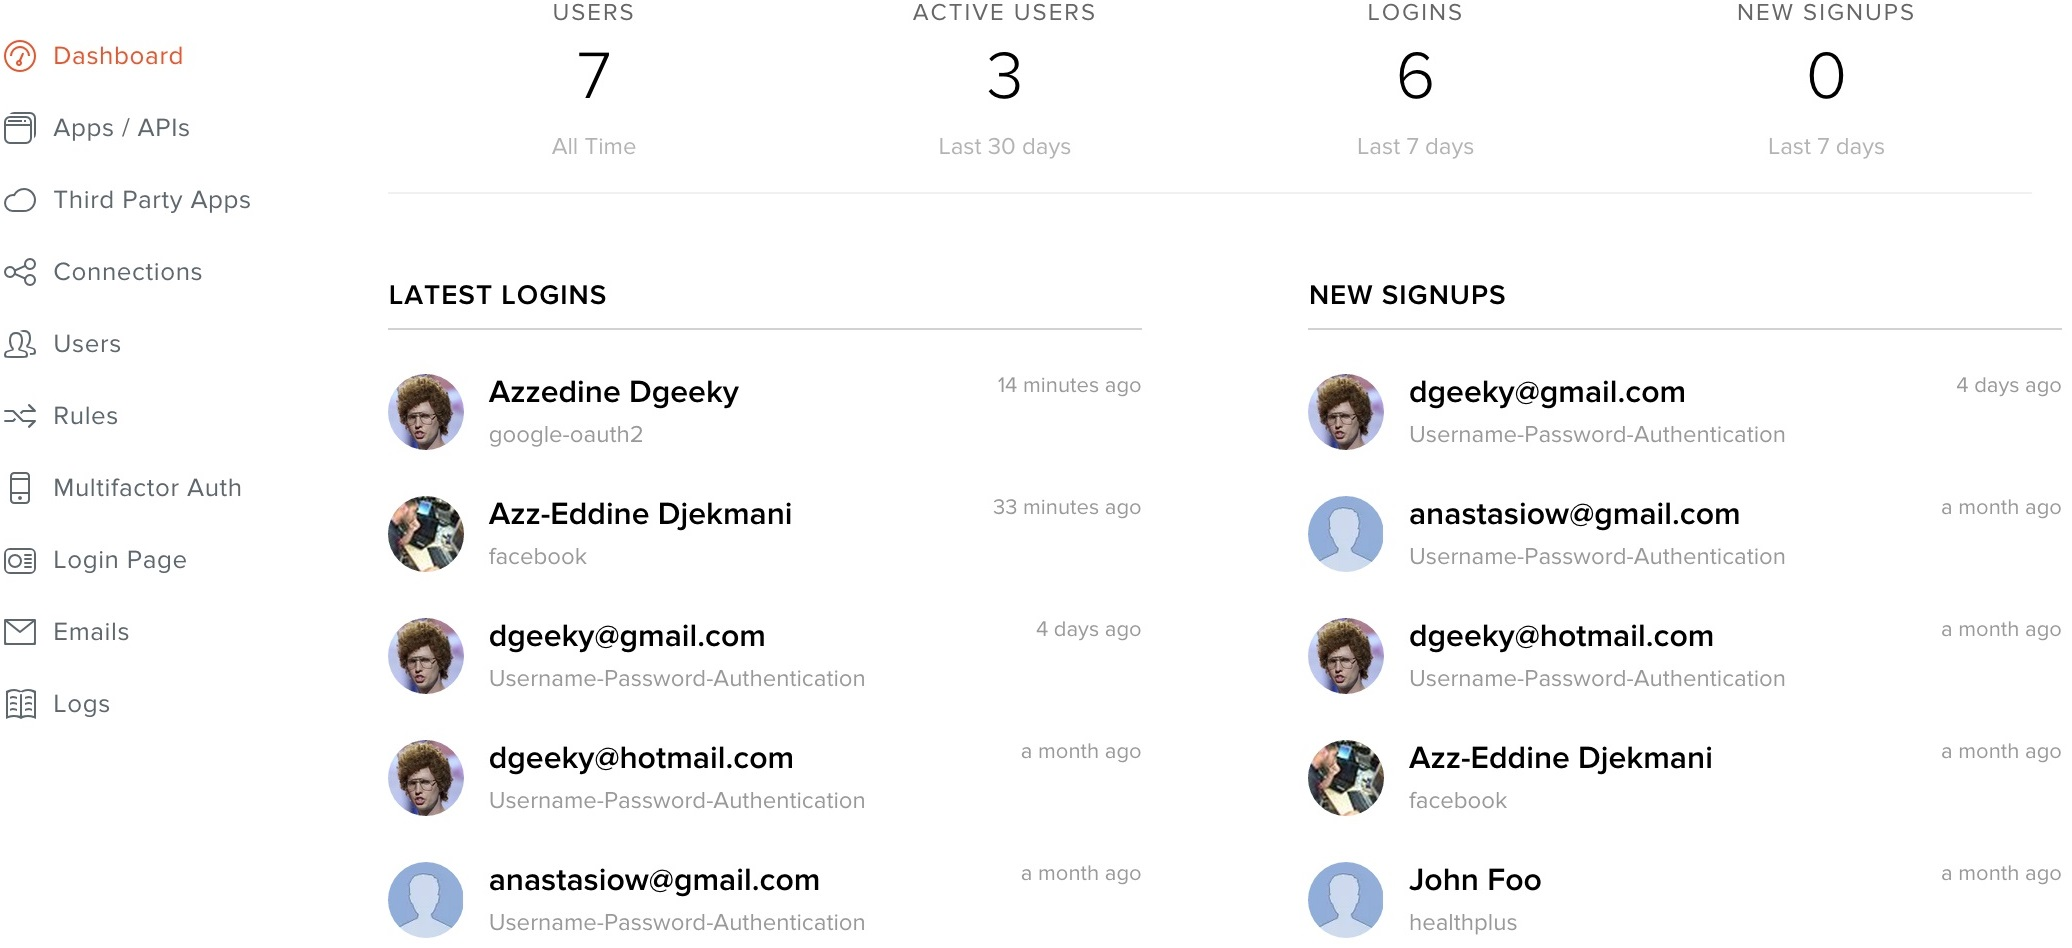
\includegraphics[scale=0.31]{e1.jpg}
\caption{Panneau de supervision des authentifications}
\label{e1}
\end{center}
\end{figure}

\vspace{6pt}
\paragraphmark

Nous pouvons aussi voir les détails de chaque connexion ou tentative de connexion à l’aide de la gestion des logs qui sont sous format JSON qui est facile à analyser et à manipuler comme indiqué dans la figure \ref{e2}:

\newpage

\begin{figure}[!ht]
\begin{center}
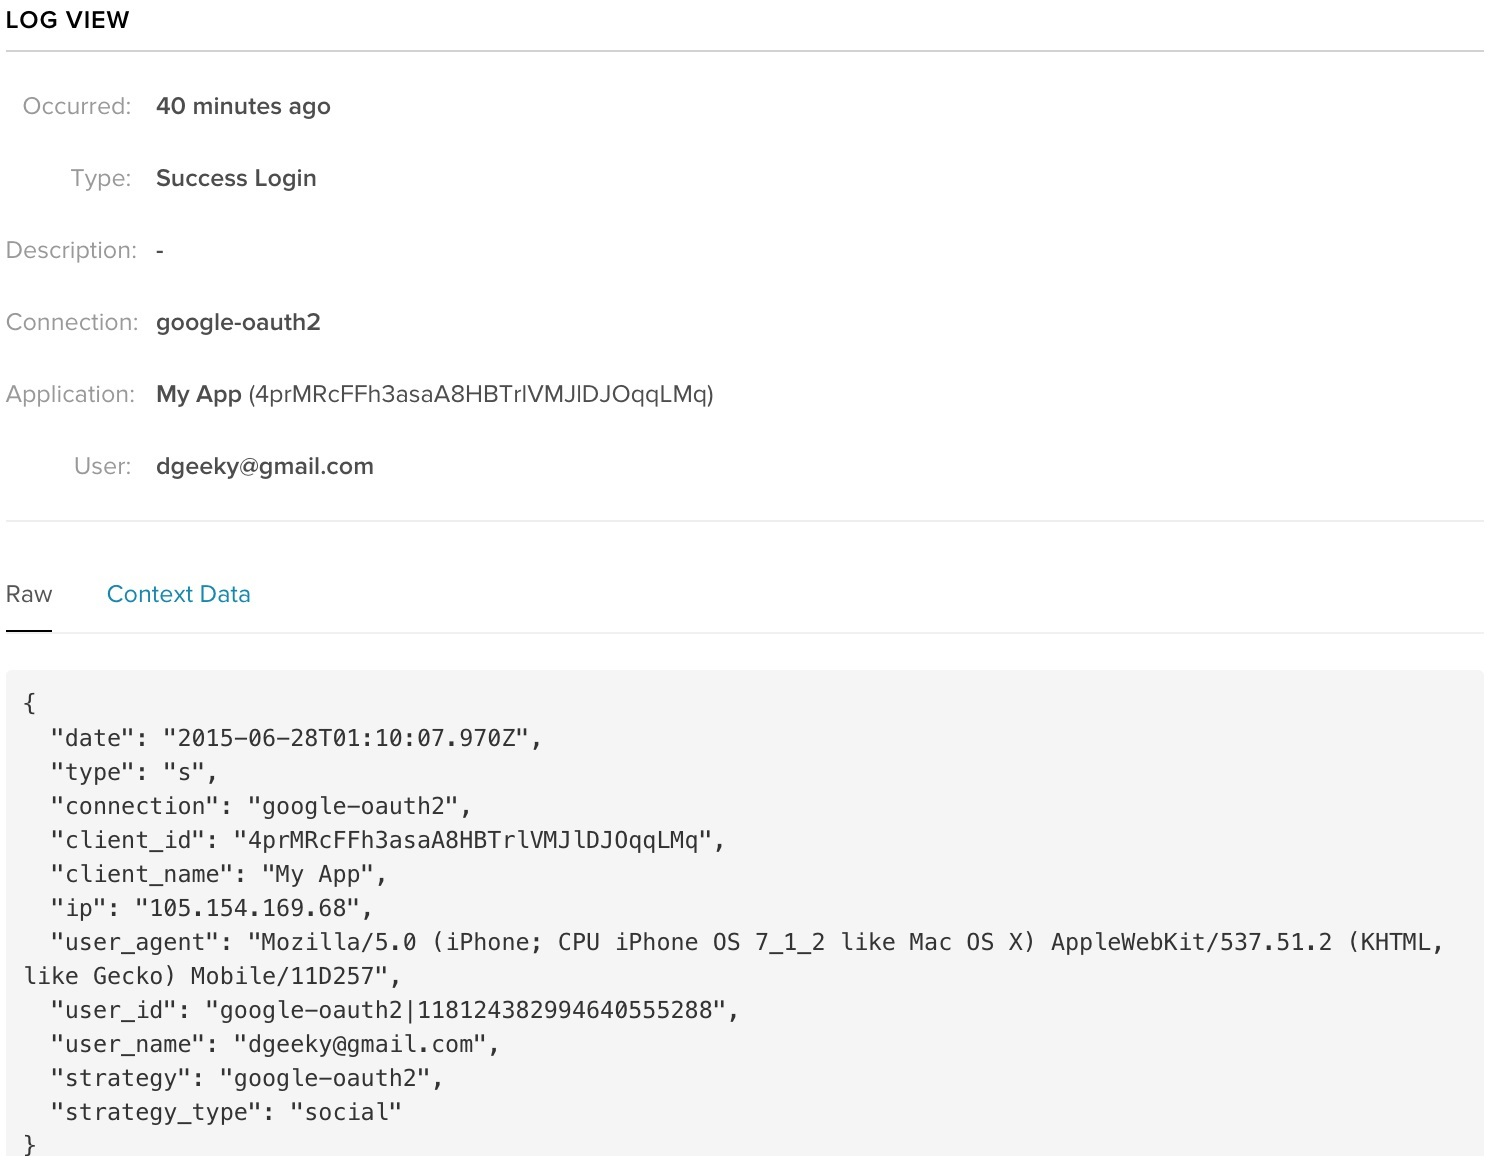
\includegraphics[scale=0.38]{e2.jpg}
\caption{Gestion des logs de connexion}
\label{e2}
\end{center}
\end{figure}

Ce mécanisme est très sécurisé. Il est à la fois anti brute force et impose aux utilisateurs d'utiliser des mots de passe forts.

\vspace{6pt}
\paragraphmark

\textbf{Anti brute force}: l'application peut contrer toutes les attaques de type brute forces. La figure \ref{e3} montre la configuration qui nous le permet:

\begin{figure}[!ht]
\begin{center}
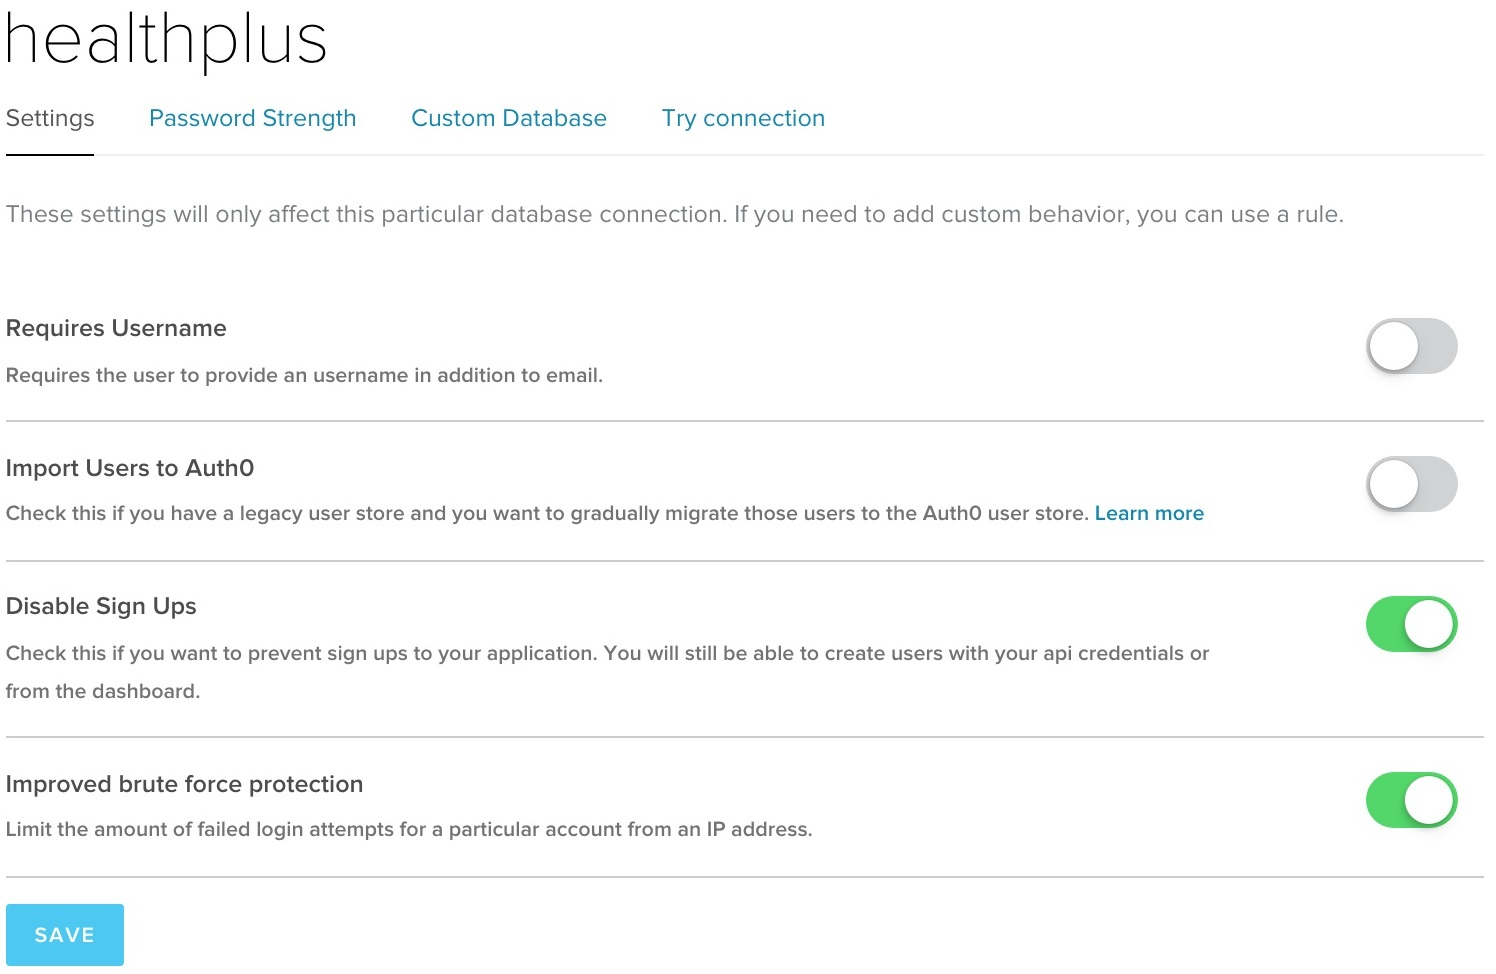
\includegraphics[scale=0.28]{e3.jpg}
\caption{Application anti brute force}
\label{e3}
\end{center}
\end{figure}

\textbf{Mots de passe forts}: l'application impose aux utilisateurs d’utiliser des mots de passe forts respectant les instructions du guide de l’OWASP comme indiqué par la figure \ref{e4} :


\begin{figure}[!ht]
\begin{center}
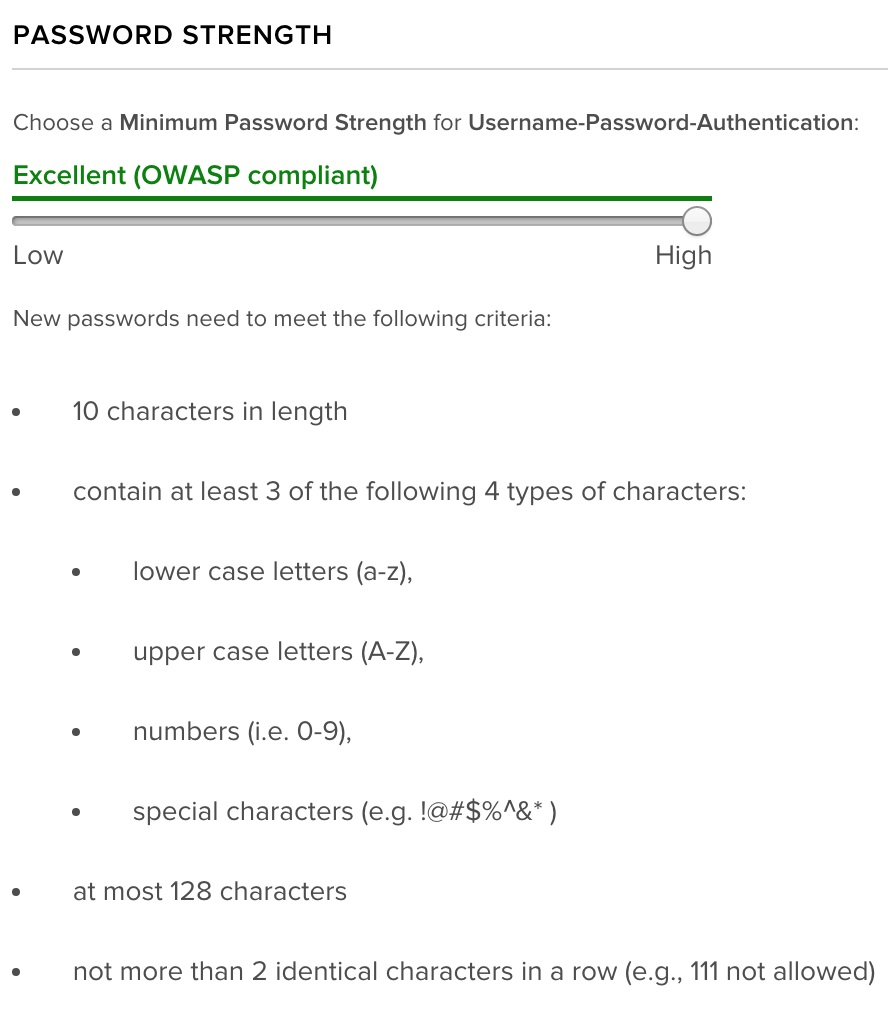
\includegraphics[scale=0.4]{e4.jpg}
\caption{Caractéristiques des mots de passe acceptés par l’application}
\label{e4}
\end{center}
\end{figure}

L'application fournit deux types majeurs d’authentification qui sont:

\begin{itemize}
	\item Authentification à l’aide d’un login (un email) et un mot de passe dont le stockage se fait sur le cloud.
	\item Connexion à travers les réseaux sociaux: Pour faciliter l’authentification, le patient peut choisir de s'authentifier à l’aide d'un réseau social (Facebook, Google+,..etc). Cette connexion permet à l'application d’obtenir les informations sur le patient depuis son compte Facebook, Google ou d’autres comme montre la figure \ref{e5} ci-dessous:
	
	\newpage

\begin{figure}[!ht]
\begin{center}
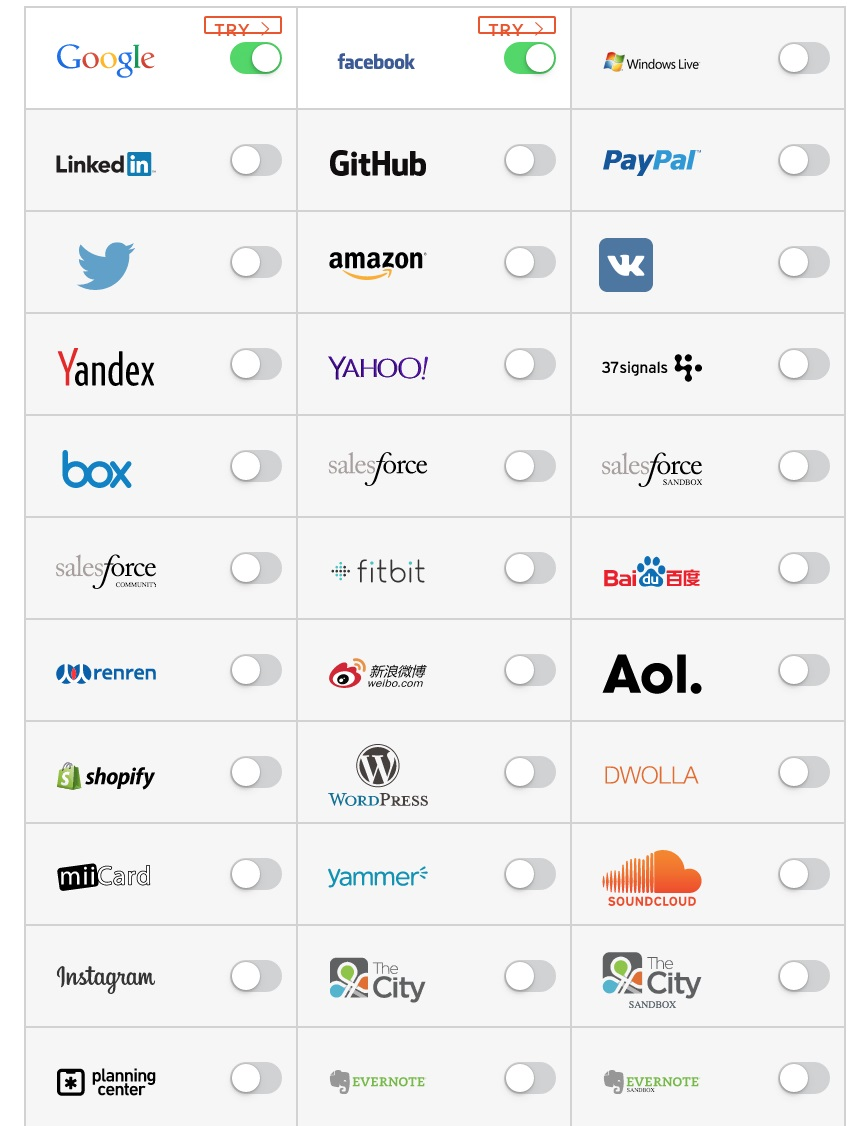
\includegraphics[scale=0.3]{e5.jpg}
\caption{Configuration des connexions depuis l’interface d’administration de Auth0}
\label{e5}
\end{center}
\end{figure}
\end{itemize}

La figure \ref{e5} ci-dessus, indique les types de connexions configurables à partir de l'interface d'administration de Auth0. Pour notre application, les connexions via Facebook et Google sont les seules autorisées.

\vspace{6pt}
\paragraphmark

L’interface d’authentification de l'application est présentée par la figure \ref{login}:

\begin{figure}[!ht]
\begin{center}
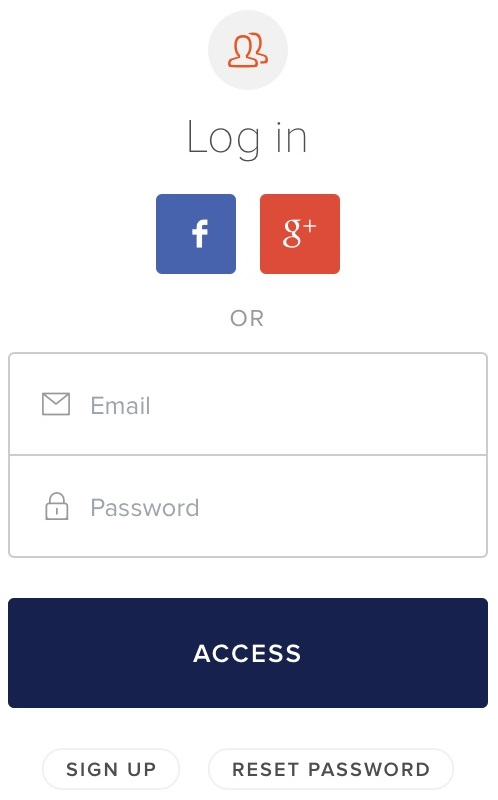
\includegraphics[scale=0.33]{login.jpg}
\caption{Interface d’authentification}
\label{login}
\end{center}
\end{figure}

Comme cité précédemment, le patient a le choix de s'authentifier à l'aide de son login (email) et son mot de passe, ou bien via un réseau social (figure \ref{login}).

\subsection{Mécanisme de privacy}

L'application utilise l'approche PPAMH afin de permettre aux patients de contrôler la divulgation de leurs renseignements personnels. Cette protection varie selon le type de groupe du patient déterminé en utilisant l'algorithme ci-dessous (figure \ref{code}):

\begin{figure}[!ht]
\begin{center}
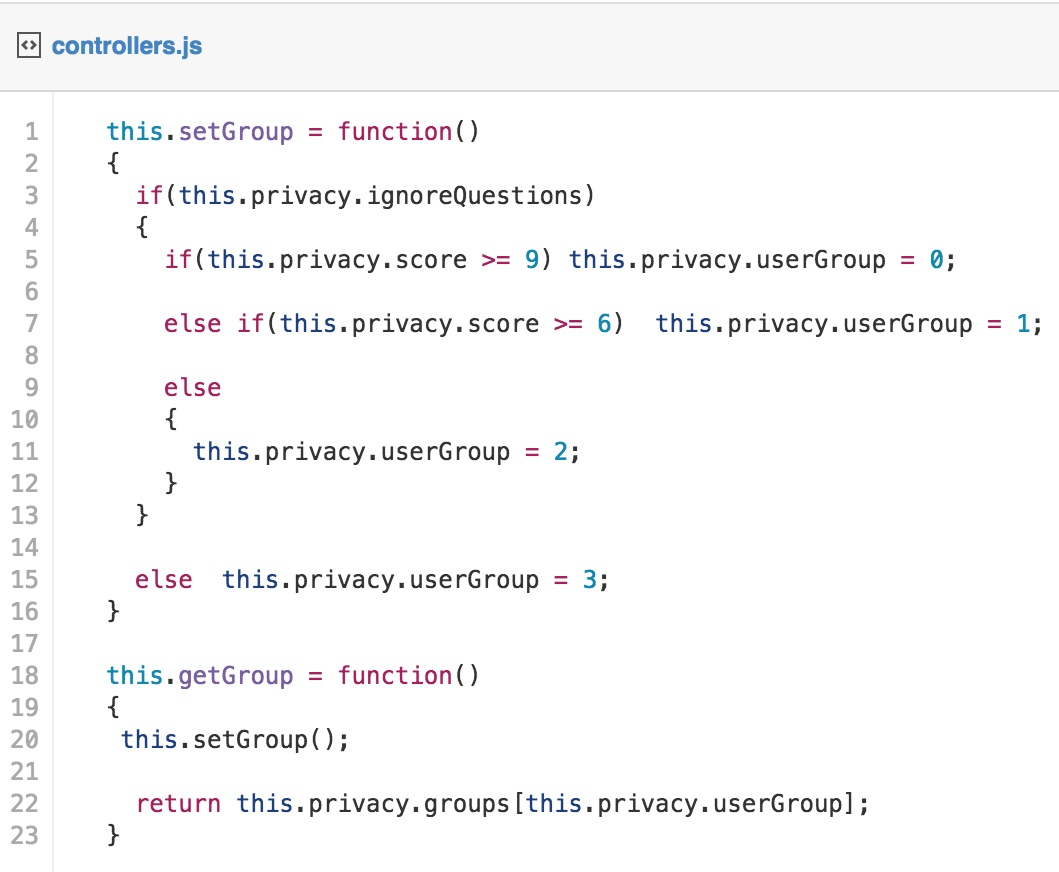
\includegraphics[scale=0.55]{code.jpg}
\caption{Algorithme de détermination de groupes}
\label{code}
\end{center}
\end{figure}

Ce code source, qui est une implémentation de l'algorithme se trouvant dans $[8]$, est écrit en Javascript.

\vspace{6pt}
\paragraphmark

Pour utiliser cet algorithme (seulement après la première authentification réussie), nous avons besoin d'un nombre entier représentant le résultat des réponses du patient au questionnaire indiqué par la figure \ref{privacy} suivante :


\newpage

\begin{figure}[!ht]
\begin{center}
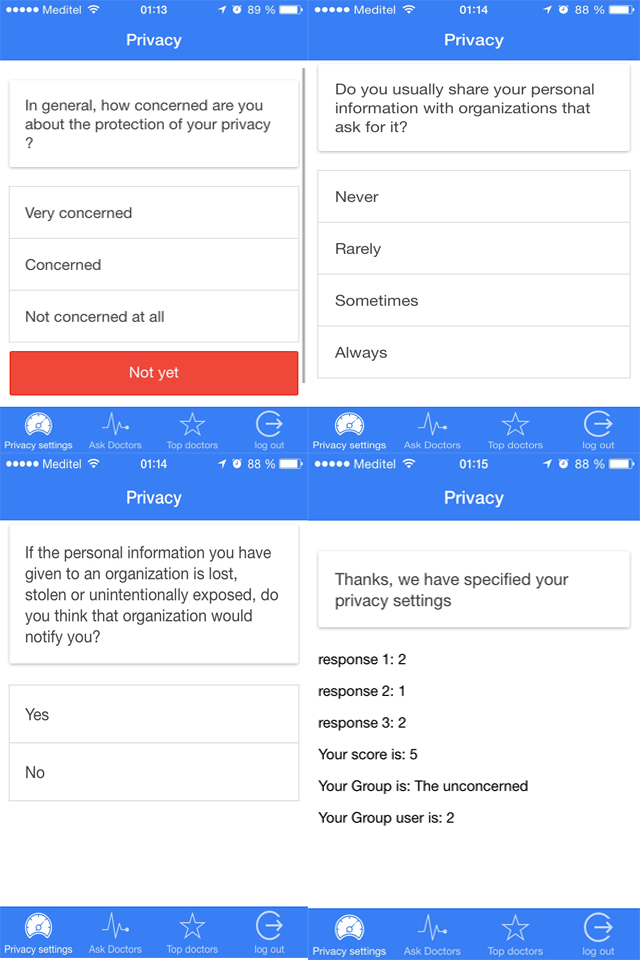
\includegraphics[scale=0.6]{privacy.jpg}
\caption{Questionnaire pour déterminer le niveau de privacy de l’utilisateur}
\label{privacy}
\end{center}
\end{figure}

Le questionnaire est constitué de trois questions indiquées dans la figure \ref{privacy}. Le patient a le choix de répondre à trois, deux, une ou aucune question et dans tous les cas un nombre entier sera calculé pour déterminer par la suite le groupe du patient en utilisant l'algorithme de la figure \ref{code}.

\subsection{Les divers services offerts par l’application}

A ce stade, les fonctionnalités principales de l'application sont réalisées et les besoins de sécurité et de confidentialité sont assurées. Pour enrichir l'application, nous ajoutons quelques fonctionmalités secondaires pour aider le patient à mieux comprendre la maladie et ses traitements.

\vspace{6pt}
\paragraphmark

Nos patients peuvent consulter les réponses des médecins experts à des questions fréquentes et d’avoir accès à une liste des meilleurs médecins de l’US et leurs coordonnées filtrés par spécialité. Cela est possible grâce à l'utilisation de la base de données d’une application d'e-santé nommée Healthtap.

\vspace{6pt}
\paragraphmark

La figure ci-dessous montre l’interface de recherche de réponses (figure \ref{rep}):

\begin{figure}[!ht]
\begin{center}
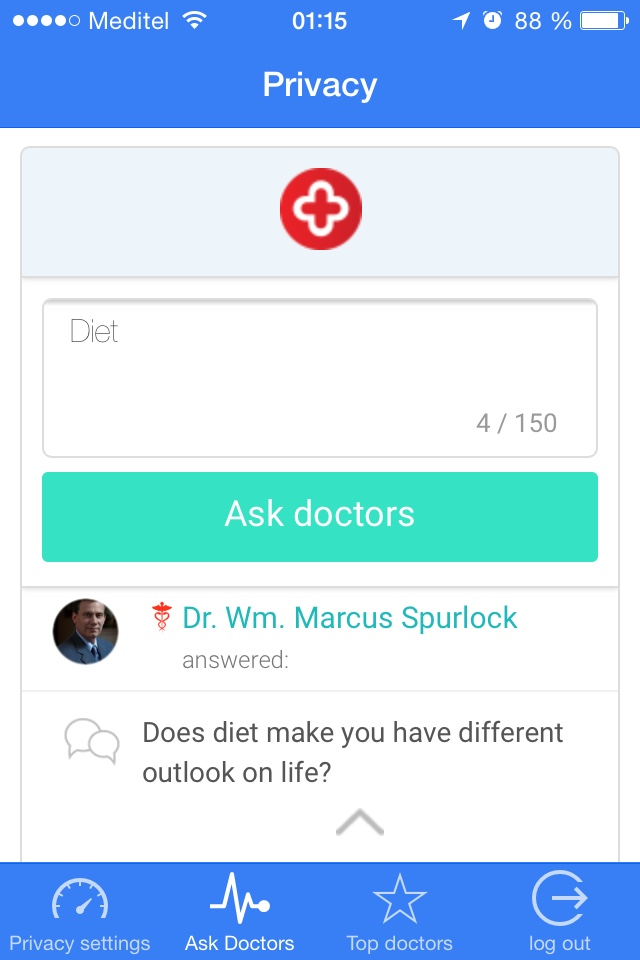
\includegraphics[scale=0.4]{rep.jpg}
\caption{Interface de recherche de réponses}
\label{rep}
\end{center}
\end{figure}

Cette interface permet à un patient de poser une question (maximum 150 caractères) et de consulter les réponses à d'autres questions.

\newpage

Les patients peuvent aussi consulter les meilleurs médecins comme le montre la figure \ref{top} ci-dessous:

\begin{figure}[!ht]
\begin{center}
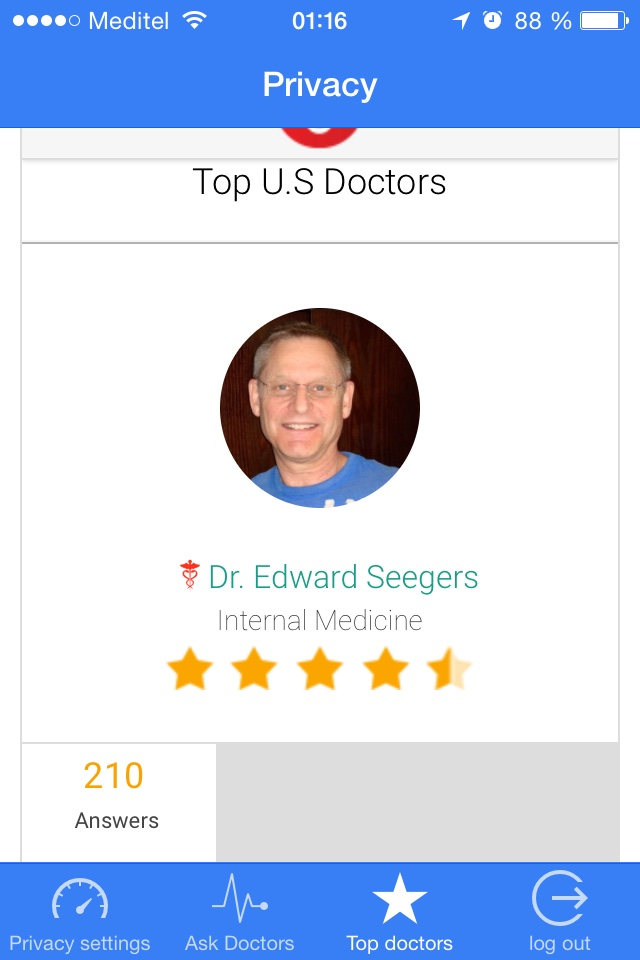
\includegraphics[scale=0.3]{top.jpg}
\caption{Interface top US docteurs}
\label{top}
\end{center}
\end{figure}

Cette recherche peut être faite par spécialité afin d'accèder aux informations pertinentes le plus rapidement possible.

\subsection{Améliorations envisagées}

Nous avons l’intention de continuer à développer cette application afin de la mettre en ligne pour la voir évoluer en situation réelle et d'évaluer ses bénifiques en terme de préservation de la vie privée des patients. Pour cela, nous devons compléter la version actuelle et enrichir les fonctionnalités déja présentes.

\vspace{6pt}
\paragraphmark

La première amélioration sera d’ajouter d'autres mécanismes d'authentification comme l'empreinte digitale afin d'adapter ce mécanisme au maximum aux différents types de patients. Nous envisageons aussi d’améliorer le questionnaire de détermination du groupe en le proposant sous d'autres formes (par exemple les réponses possibles sous forme des images).

\vspace{6pt}
\paragraphmark

Enfin, il serait bénifique de développer une version de l'application pour les smartphones utilisant Windows Phone comme système d'exploitation afin d'augementer le nombre de nos clients. 